\documentclass[a4paper,11pt]{article}
\usepackage[utf8]{inputenc}
\usepackage[spanish]{babel}
\usepackage[a4paper]{geometry} 
\usepackage{parskip}
\usepackage[hidelinks]{hyperref} 
\usepackage{graphicx} 
\usepackage{url}     
\usepackage{xcolor} 
\usepackage{fullpage}
\usepackage{float}
\usepackage{caption}
\usepackage{enumitem}
\usepackage{subcaption}

\captionsetup{font={bf,tiny}}
\setlist[enumerate]{parsep=1.5pt}


\title{Informe de integración Rasa-LLM}
\author{Pablo Valenzuela Álvarez}
\date{\today} 

\begin{document}
	
	\maketitle
		
	\section{Introducción}
	
		En los últimos años, el desarrollo de modelos de lenguaje de gran escala (LLMs, por sus siglas en inglés) ha revolucionado la forma en que las máquinas procesan y generan lenguaje natural. Estos modelos, entrenados con enormes volúmenes de datos, han demostrado capacidades avanzadas en comprensión contextual, generación de respuestas y mantenimiento de conversaciones coherentes.  
		
		Por otro lado, \textbf{Rasa} se ha consolidado como una de las principales plataformas de desarrollo de asistentes conversacionales, ofreciendo un marco flexible basado en procesamiento de lenguaje natural y aprendizaje automático. Sin embargo, los modelos tradicionales de Rasa se basan en arquitecturas específicas de clasificación de intenciones y gestión de diálogos, lo que puede limitar su capacidad para comprender consultas complejas o responder de manera más natural.  
		
		En este contexto tenemos \textbf{Rasa Pro}, la versión empresarial de Rasa, que ha incorporado funcionalidades avanzadas para aprovechar las capacidades de los LLMs. Una de sus innovaciones clave es \textbf{CALM} (Conversational AI with Language Models), un enfoque que combina la flexibilidad de Rasa para gestionar diálogos estructurados con la potencia de un modelo de lenguaje. Esta integración permite generar respuestas más naturales y contextualizadas, mejorar la comprensión de entradas ambiguas y reducir el tiempo de entrenamiento.
		
		El objetivo de este informe, es valorar el uso de esta nueva herramienta, teniendo en cuenta las ventajas y desventajas que ofrece respecto a otras soluciones de código abierto disponibles.
		
	\section{Desarrollo}
	
		En esta sección vamos a enumerar ciertos aspectos que ofrece esta herramienta, comparandola además con otros productos de código abierto que hay en el mercado.			
			
		\subsection{Licencia de uso}
			
			Uno de los principales inconvenientes a considerar al evaluar el uso de este producto es su licencia de uso. Dado que Rasa Pro está diseñado para entornos empresariales, está sujeto a restricciones específicas. Es posible obtener una licencia para desarrolladores de forma gratuita a través del sitio web oficial de Rasa (\textcolor{blue}{\href{https://rasa.com/docs/rasa-pro/}{enlace}}) \cite{01_RasaProIntro}, pero esta licencia presenta ciertas limitaciones que detallamos a continuación:
			
			\begin{enumerate}
				\item Límite de 1000 conversaciones mensuales (100 para asistentes internos dirigidos a empleados).
				\item Uso restringido a un único usuario.
				\item Permite su uso en entornos comerciales, pero con restricciones específicas definidas en la licencia.
				\item Cada clave de licencia tiene una validez de 12 meses.
			\end{enumerate}
			
			Existen dos problemas clave derivados de estas restricciones. En primer lugar, aunque la licencia es gratuita, requiere renovación anual, lo que puede suponer una limitación a largo plazo. En segundo lugar, el límite de conversaciones mensuales es demasiado bajo para las necesidades de nuestro proyecto, lo que representa una desventaja en comparación con otras soluciones de código abierto, que no imponen restricciones de uso y son completamente gratuitas.
			
		\subsection{Facilidad de uso}
		
			Partiendo de que ya conocemos la estructura y el codigo que se usa en Rasa, observamos que con Rasa Pro se han prescindido de algunos archivos, pero la estructura sigue siendo la misma (ver figura \ref{fig:01-comparacionEstructuras}).
			
			\begin{figure}[H]
				\centering
				\begin{subfigure}{0.45\textwidth}
					\centering
					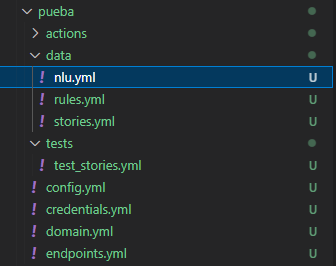
\includegraphics[height=5cm]{img/00-estructuraRasa.png}
					\caption{Estructura de Rasa}
				\end{subfigure}
				\hspace{0cm}
				\begin{subfigure}{0.45\textwidth}
					\centering
					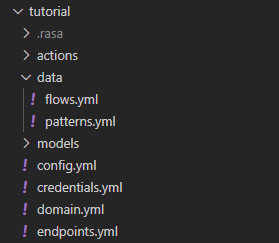
\includegraphics[height=5cm]{img/01-estructuraRasaPro.png}
					\caption{Estructura de Rasa Pro}
				\end{subfigure}
				\caption{Comparación de las dos estructuras}
				\label{fig:01-comparacionEstructuras}
			\end{figure}
			
			Los archivos \textit{nlu.yml}, \textit{rules.yml} y \textit{stories.yml} han sidos sustituidos por \textit{flows.yml} y \textit{pattern.yml}. El contenido de estos archivos es el flujo de conversación que el asistente tiene que seguir ante un determinado input del usuario (ver figura \ref{fig:02-contenidoFicheros}).
			
			\begin{figure}[H]
				\centering
				\begin{subfigure}{0.45\textwidth}
					\centering
					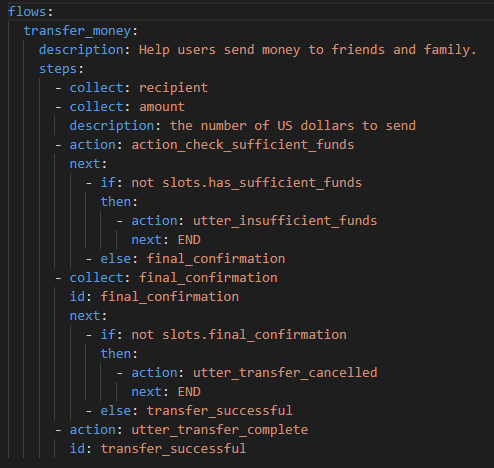
\includegraphics[width=0.8\textwidth]{img/02-flows.png}
					\caption{flows.yml}
				\end{subfigure}		
				\hspace{0cm}		
				\begin{subfigure}{0.45\textwidth}
					\centering
					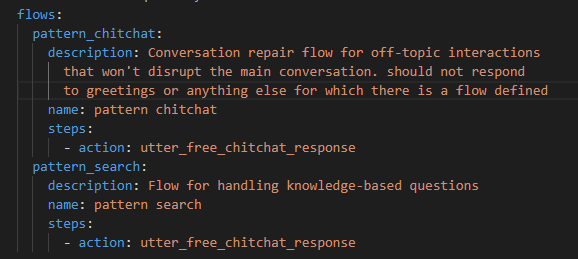
\includegraphics[width=1\textwidth]{img/03-patterns.png}
					\caption{patterns.yml}
				\end{subfigure}
				\caption{Contenido de los ficheros}
				\label{fig:02-contenidoFicheros}
			\end{figure}
			
			Los flujos están diseñados para recoger la información necesaria para realizar el proceso que tienen determinado. Gracias a la etiqueta \textit{collect} se guarda el valor recogido en un \textit{slot} de Rasa. La etiqueta \textit{description} ayuda al modelo a manejar mejor la respuesta dada al usuario.
			
			Los Slots y respuestas se manejan igual y están situadas en el mismo lugar que en la versión normal de Rasa (\textit{domain.yml}), aunque también es posible añadir a las respuestas un \textbf{prompt} (ver figura \ref{fig:03-respuestaPrompt}).
			
			\begin{figure}[H]
				\centering
				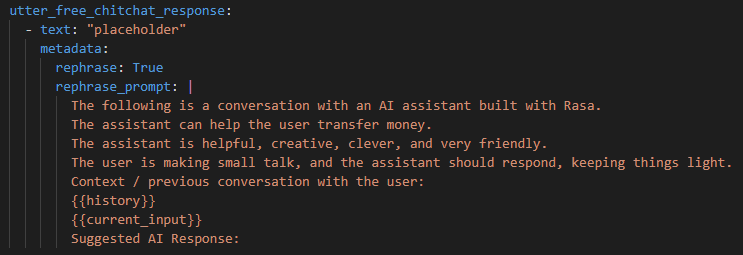
\includegraphics[width=0.8\textwidth]{img/04-respuestaPrompt.png}
				\caption{Respuesta con prompt.}		
				\label{fig:03-respuestaPrompt}
			\end{figure}
			
			Por lo que podemos observar, ya no disponemos de \textit{intents} en esta versión, ya que estos son deducimos automáticamente por el modelo de lenguaje. Respecto al código, es claro y fácil de modificar para adaptarlo  a las necesidades de cualquier proyecto o empresa, y cuenta con la posibilidad de controlar las respuestas dadas por el asistente dado a que todo el código permanece \textbf{on premise}. También permite la conexión con modelos de lenguaje locales, pero ese tema se abordará en la siguiente subsección.
		
		\subsection{Rendimiento}
		
			El asistente de prueba usa un modelo desarrollado por Rasa (\textcolor{blue}{\href{https://huggingface.co/rasa/cmd_gen_codellama_13b_calm_demo}{enlace}}) \cite{02_codellama} que ya esta preparado para ser usado en asistentes desarrollados bajo el enfoque \textbf{CALM}, es decir, que traduce los mensajes enviados por el usuario en los comandos que son necesarios para avanzar en la conversación. De acuerdo a la documentación, este modelo no es capaz de generar texto arbitrario, ni texto problemático o dañino.
			
			A la hora de probar el asistente, Rasa Pro incluye un herramienta muy interesante: el \textbf{inspector}. Gracias a ella, podemos seguir el flujo de la conversación de manera visual gracias a un grafo que se actualiza automáticamente mientras estamos conversando con el asistente (ver figura \ref{fig:04-grafoFlujo}).
			
			\begin{figure}[H]
				\centering
				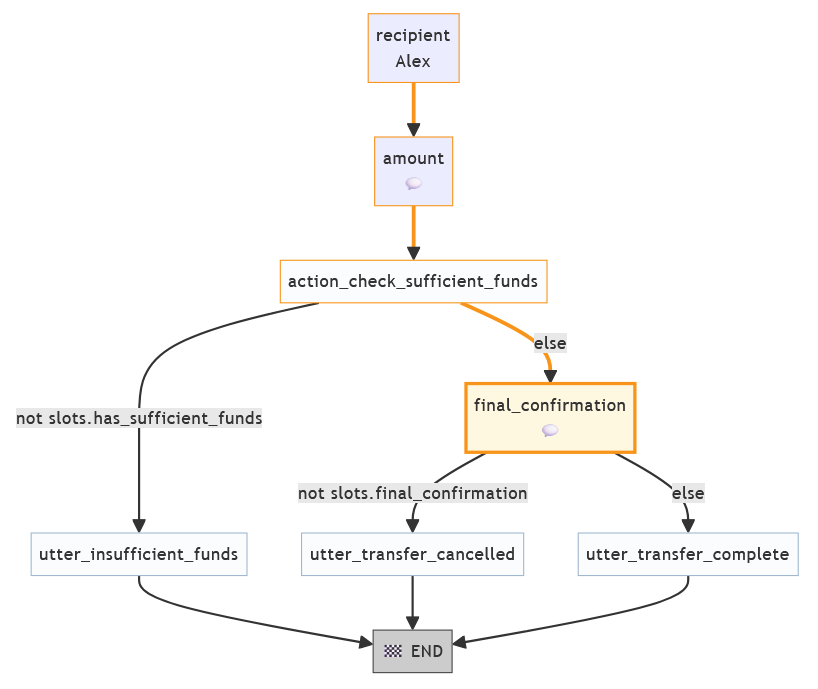
\includegraphics[width=0.8\textwidth]{img/05-grafoFlujo.png}
				\caption{Grafo con el flujo de la conversación.}		
				\label{fig:04-grafoFlujo}
			\end{figure}
			
			En las conversaciones podemos optar por dar los datos uno a uno o todos a la vez. Puede controlar este tipo de entrada de datos al igual que la versión de normal Rasa (ver figura \ref{fig:05-conversacion}).
			
			\begin{figure}[H]
				\centering
				\begin{subfigure}{0.45\textwidth}
					\centering
					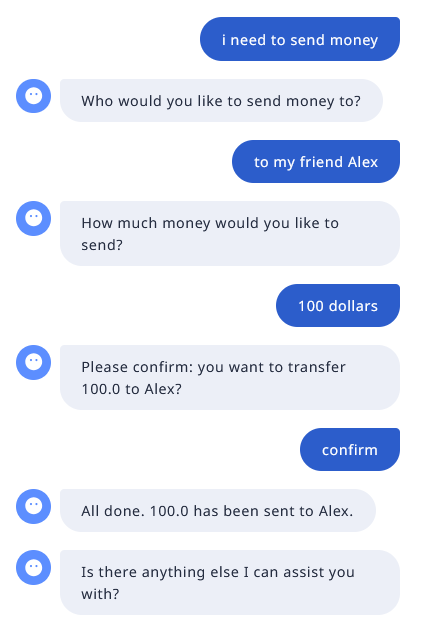
\includegraphics[width=0.8\textwidth]{img/06-conversacion1.png}
					\caption{Datos uno a uno}
				\end{subfigure}		
				\hspace{0cm}		
				\begin{subfigure}{0.45\textwidth}
					\centering
					\includegraphics[width=1\textwidth]{img/07-conversación.png}
					\caption{Todos los datos a la vez}
				\end{subfigure}
				\caption{Tipos de conversaciones soportadas}
				\label{fig:05-conversacion}
			\end{figure}
				
			El rendimiento de este modelo es prácticamente inmediato, lo que lo convierte en una opción a considerar. Sin embargo, como mencionamos anteriormente, este modelo no genera respuestas arbitrarias y, dependiendo de la lógica de negocio requerida, podría no ser la opción más adecuada.  
			
			Rasa Pro permite modificar el modelo de lenguaje dentro de la configuración del proyecto, ofreciendo compatibilidad con modelos tanto locales como en la nube, incluyendo OpenAI y otras alternativas.  
			
			En nuestras pruebas, utilizamos un modelo local a través de \textbf{Ollama}, específicamente \textit{llama3.2}. Sin embargo, los resultados obtenidos no fueron óptimos. Además de presentar tiempos de respuesta significativamente más altos en comparación con el modelo anterior, en algunas ocasiones omitía pasos dentro de la conversación.  
			
			Por último, no pudimos realizar pruebas con los modelos de OpenAI, ya que no disponíamos de una clave de acceso a su API en el momento de la evaluación. Esto impidió comparar su rendimiento y calidad de respuesta frente a las otras opciones probadas.
	
	\section{Conclusión}
	
		La integración de Rasa Pro con modelos de lenguaje representa un avance significativo en el desarrollo de asistentes conversacionales. La adopción del enfoque \textbf{CALM} permite gestionar diálogos de manera más dinámica, eliminando la necesidad de definir intenciones explícitas y mejorando la experiencia del usuario.  
		
		Sin embargo, a pesar de sus ventajas, Rasa Pro presenta algunas limitaciones que deben considerarse. En primer lugar, las restricciones impuestas por su licencia pueden dificultar su uso en proyectos con una alta demanda de interacciones, especialmente en comparación con otras soluciones de código abierto sin restricciones de uso. En segundo lugar, aunque el modelo de lenguaje proporcionado por Rasa Pro ofrece un rendimiento inmediato y una integración optimizada, su capacidad de generación de respuestas sigue siendo limitada y no siempre se ajusta a todos los casos de uso.  
		
		En nuestras pruebas, el uso de modelos de lenguaje locales a través de \textbf{Ollama} no logró resultados satisfactorios debido a tiempos de respuesta más elevados y a ciertas inconsistencias en la generación de respuestas. Además, no pudimos evaluar los modelos de OpenAI debido a la falta de acceso a una clave de API en el momento de la prueba, lo que impidió realizar una comparación más completa.  
		
		En conclusión, Rasa Pro se presenta como una opción potente y viable para la implementación de asistentes conversacionales en entornos empresariales, especialmente para aquellos que buscan mantener el control del procesamiento de datos en local. No obstante, su idoneidad dependerá de las necesidades específicas del proyecto y de las limitaciones impuestas por su modelo de licencia. Para escenarios que requieran un mayor volumen de interacciones o una mayor capacidad de generación de texto, pueden considerarse alternativas más flexibles dentro del ecosistema de código abierto.  
		
		\newpage		
		\bibliographystyle{unsrt}  
		\bibliography{bibliografia}
	
\end{document}
